\begin{frame}{Replication of ``Business Cycle Anatomy''}
    
    \label{replication-slide}

    Large VAR with 10 variables

    \vspace{0.5cm}

    \textbf{Identification scheme:}

    Choose the linear combination of empirical shocks that explains the most forecast error variance in a target variable, at a target frequency.

    \vspace{0.5cm}

    In particular, Angeletos et al. choose to target unemployment at the ``business cycle frequency'' of $\frac{2 \pi}{32}$ to $\frac{2 \pi}{6}$, which matches a period of 6 to 32 quarters. 

\end{frame}


\begin{frame}{Replication of ``Business Cycle Anatomy''}

    \begin{figure}
        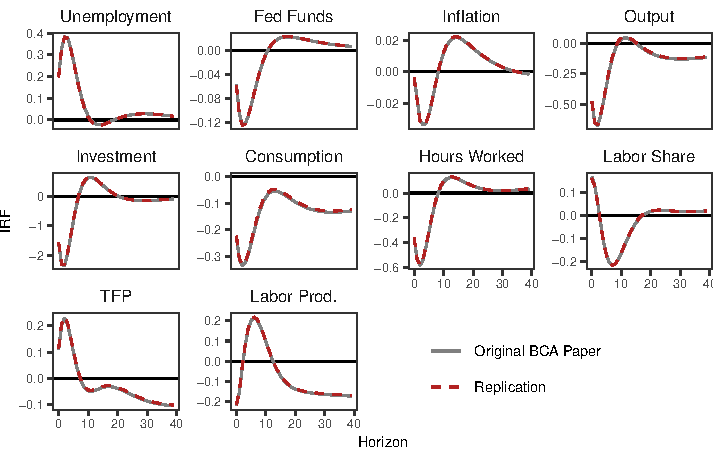
\includegraphics[height = 3in]{figs/fig1_bca_replication.pdf}
    \end{figure}

\end{frame}
